\documentclass[10pt,a4paper]{article}
%You comment with the modulo-sign. Before the \begin keyword you put what packages
%you want to use etc. If you want to include graphics for example you need the graphicX-package
\usepackage{graphicx}
\usepackage{amsmath}
\usepackage[utf8]{inputenc}
\usepackage{float}
\usepackage[none]{hyphenat}
%You also define your title here. You create a title by putting maketitle after you have begun the document
\title{Requirements Specification - v.1.1}
\author{\begin{large}{Robotics Safety}\end{large}\\\\
Olle Fridolfsson (ollfr940) \\  Niklas Hansson (nikha310) \\ Patrik Hillgren (pathi747) \\ Benjamin Ingberg (benin542)\\ Pär Lundgren (parlu048) \\ Mattias Nilsson (matni796)}
\setlength{\parindent}{0cm}	%This removes the automatic indentation
\begin{document}
\maketitle
%Latex keeps track of your sectioning automatically. To get a table of contents just put
\centerline {Responsible editor: Olle Fridolfsson}
\newpage
\tableofcontents
%To get a new page just put
\newpage
\noindent %Just makes it so that the first paragraph isn't indented
\section{Introduction}
This document specifies the requirements for the Robotics Safety project that is a part of the course TSBB11 at LiU, held at CVL.
\section{Purpose and goal}
The purpose of the project is to develop a system that monitors the surrounding of industrial robots and allows humans to safely work side-by-side with them. 
The goal is to provide a system that meets the expectation of Yaskawa Nordic AB.
The requirements of the project are all assigned to different sprints. The sprints are vividly defined and can be changed depending on how much time the different requirements take to fulfill. 

\section{Definitions}
There are predefined safety zones for the surrounding of the robot and these will be used to decide whether the robot should continue to work as normal, slow down its working pace or simply stop.

\section{System Overview}
The system will consist of at least one kinect sensor that sends a depth image and a colour image to the computer. Together with geometric data about the robot from the controller it is possible to detect if any object is entering the region of interest.

\begin{figure}[H] 
  \centering
    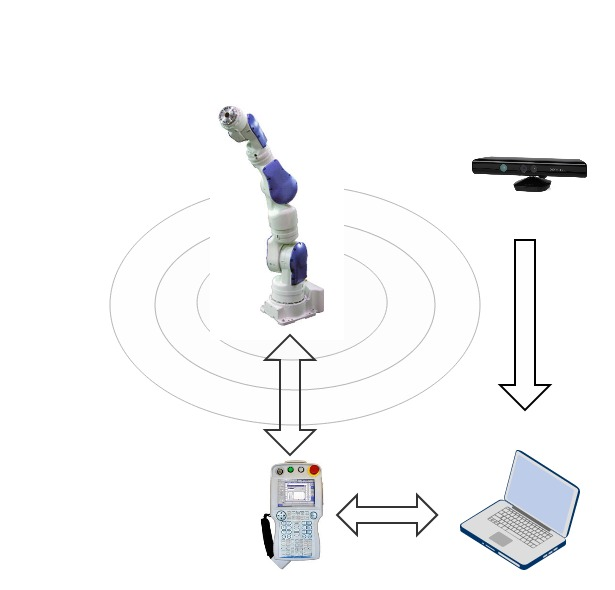
\includegraphics[width = 0.7\textwidth]{robot.jpg}
    \caption{A picture of the robot, the kinect camera and the connecting computer.}
    \label{fig:safetyzone}
\end{figure}


\section{Requirements}
The requirements of the project are listed below. If a requirement is planned to be solved in a specific sprint, it is marked with the number of that sprint. 
{\addtolength{\leftskip}{10mm}
\subsection{Product Requirements}
This section describes the requirements of the finished product. These are the overall goals of the project. \par}

\begin{enumerate}
\item Alarm when an object approaches robot.

There will be three different zones around the robot. If a human is detected in zone 1, closest to the robot, a red marker will be visualized to signal extreme caution. In zone 2 the marker will be of color yellow and in zone 3 the marker is green.

%\item Control of the robots working pace with respect to the closest moving object, sprint 3.
%
%{\addtolength{\leftskip}{5mm}The robot will slow down if a human being is approaching it and stop if someone gets to close.
%\\\\The safety zones are dynamical and will deform depending on the robot's orientation and speed. \par}

%\item Evaluation of the product's performance and reliability using an automatic system, sprint 4.

\subsection{System Interfaces}
These section describes how the functionality of the of the program will be split into modules.

\item There will be a module for segmentation of moving objects using statistical background models, sprint 2.

{\addtolength{\leftskip}{5mm}It will be important to know what in the depth image is background and what are objects. To know this, object segmentation is needed. In this project, statistical background modelling will be used.\par}

\item There will be a module for generating a 3D-model from robot data,\\ sprint 2.
 
{\addtolength{\leftskip}{5mm}The robot will give information about its orientation. This module will take that information and generate a 3D-robot model.\par}
 
\item There will be a module for linking data from the 3D-robot model and the results from the segmentation of the depth image, sprint 3.

{\addtolength{\leftskip}{5mm}This module distinguishes the robot from other moving objects in the images. This will be possible since a calibration between the coordinate system of the robot and the camera will be done. If it is necessary the colour of the robot will also be used to distinguish the robot from other moving objects.\par}


\item There will be a module for evaluation of the complete system, sprint 4.

{\addtolength{\leftskip}{5mm}This module will compute distances to moving objects and determine in which safety zone an object is. From this there will be possible to display the number of moving objects in the robot's environment. 
\par}

%\item There will be a module for controlling the robot via the remote control, sprint 3.
%
%{\addtolength{\leftskip}{5mm}The robot will be controlled based on moving objects within the safety zones. This module will manage this, sending the correct signals to the robot based on what is found in the depth and color image.
%\par}

\item There will be a module for real-time visualization of all 3D-data,\\ sprint 3.

{\addtolength{\leftskip}{5mm}There will be an 2D-environment where the robot and other 3D-data is visualized.\par}

\subsection{Hardware Interfaces}

\item Camera setup specifications, sprint 2.

{\addtolength{\leftskip}{5mm} The number of cameras and their positions will be specified.\par}

\subsection{Communication Interfaces}

\item Data from the Kinect sensor should be available in the computer, \\sprint 2.
\item Data from the robot controller should be available in the computer, \\sprint 2.

\subsection{Constraints assumptions and dependencies}
These are the requirements that is assumed to be fulfilled for the system being able to work properly. None of them are categorized to a sprint.

\item The Kinect sensor should be placed in a position so that it can overview the robot. This ensures that a human being will not be able to approach the robot without entering the safety zones.

\item The system will not work in an environment that is to bright, there is an assumption of a reasonable amount of light.

\item The data used will always be the current input from camera and robot, i.e there will not be any module handling delays between inputs.

\subsection{Functional requirements}
This section describes the requirements of functionality for the subsystems and for the system in general.
\item The system will work if the kinect is placed such that occlusion is minimized. 
\item Process information from robot controller and generate 3D-data, \\sprint 2.
%\item Send control signal to the robot from computer, sprint 2.
\item Calibrate the coordinate system of the robot to the coordinate system of the Kinect, sprint 3. 

\item Link the robot's 3D-data to the 3D-data from the Kinect sensor, sprint 3.

\item Determine the distance from the robot to the other found objects, \\sprint 3.

%\item Evaluate the performance of the result automatically, sprint 4.

\item Detect a human being that is entering the area of interest, sprint 4.

\item Track objects in the image using statistical background models, sprint 2.

\end{enumerate}

\end{document}

